\section{Confronto ambienti}\label{confrontoAmbienti}
In questa sezione verranno discusse le differenze riscontrate durante l'implementazione e l'analisi dei diversi ambienti.
Si discuteranno gli aspetti riguardanti l'usabilità nella sezione \ref{usabilita} e gli aspetti prettamente legati alle performance
nella sezione \ref{analisiRisultati}.

\subsection {Usabilità}\label{usabilita}

\subsubsection{Matlab}
\paragraph{Documentazione}
Matlab è tutt'oggi un software molto utilizzato sia professionalmente, sia in ambito accademico. Il software è mantenuto e anche la sua documentazione
resta aggiornata e precisa. La documentazione, oltre che essere consultabile sul web, è facilmente reperibile all'interno dell'ambiente con l'utilizzo
della direttiva \emph{help} seguita dalla funzione per cui si vuole richiedere la documentazione.
\paragraph{Facilità d'uso}
Il software è installabile recandosi sul sito \url{https://it.mathworks.com/downloads/}. Essendo un software a pagamento è richiesta una licenza per poter usufruire dei % TODO
suoi servizi. Il suo utilizzo si è dimostrato semplice e abbastanza intuitivo avendo anche il supporto di un'ottima documentazione.
\paragraph{Community}
Un altro aspetto che è stato valutato è stato quello della community. La community di Matlab si dimostra essere molto
attiva e partecipante. Mathworks offre un servizio simile a quello offerto da \url{https://stackoverflow.com/} limitato però
esclusivamente al software di Matlab. È possibile, infatti, porre domande riguardo ad un problema riscontrato durante lo sviluppo
di un proprio script, oppure riguardo al corretto utilizzo delle funzioni offerte dal software. Gli utenti, quindi, sono resi partecipi dando
la possibilità di rispondere a queste domande aiutando e risolvendo problemi riscontrati da altre persone.
Questo strumento permette, inoltre, di condividere funzioni custom, sviluppate da utenti, che possono essere scaricate e integrate all'interno del proprio lavoro.
\paragraph{Problemi riscontrati}
Durante l'utilizzo di questo software non sono stati riscontrati particolari problemi.

\subsubsection{Octave}
\paragraph{Documentazione}
Anche GNU Octave è un software tutt'oggi mantenuto. Esso offre una documentazione ricca e aggiornata offrendo esempi e modalità d'uso delle sue funzioni.
Pur dichiarandosi strettamente compatibile con Matlab molte funzioni sembrano non essere però ancora implementate\footnote{funzioni come \emph{memory} e \emph{readtable} restituiscono \emph{"function is not yet implemented in Octave"}}.
Come Matlab, Octave offre la possibilità di consultare la documentazione online e direttamente all'interno dell'ambiente con la stessa direttiva \emph{help}
utilizzata in Matlab.
\paragraph{Facilità d'uso}
Il software è completamente open source e non ha bisogno di alcuna licenza a pagamento. Può essere scaricato gratuitamente dal sito \url{https://www.gnu.org/software/octave/download.html}.
L'installazione richiede un tempo minore rispetto a Matlab necessitando di uno spazio su disco inferiore (Da circa 5GB per Matlab a circa 2GB per Octave). % TODO
Il suo utilizzo risulta essere semplice offrendo, per quanto già detto in precedenza, la stessa sintassi di Matlab.
\paragraph{Community}
Octave, a differenza di Matlab, non offre alcuna possibilità di interagire tra utenti e problematiche riscontrate durante lo sviluppo di un proprio script.
Questo risulta in una maggiore difficoltà di ricerca di un problema, tanto da finire a consultare i forum di Mathworks. Pur essendo in gran parte compatibile,
ci sono comunque alcune differenze tra i due ambienti.
\paragraph{Problemi riscontrati}
Durante la realizzazione di questa analisi è stato necessario leggere un file csv contenente diverse tipologie di dato. Le funzioni offerte da Octave non offrono però questa possibilità costringendo nel fare l'operazione in Matlab.
Inoltre, come già accennato nella sezione \ref{fase3}, in Octave non esiste la possibilità di monitorare l'impiego di memoria RAM utilizzato per una data funzione contrariamente a come avviene in Matlab.
È stata infine riscontrata un'imprecisione nell'errore ricevuto in seguito al fallimento della decomposizione di Cholesky (Figura \ref{fig:octaveImprecisione}).
\begin{figure}[H]
\centering
\begin{verbatim} 
    warning: warning -2, at line 146 in file ../Core/cholmod_memory.c:
        out of memory
    warning: called from
        solveWithCholesky at line 2 column 9
        matrixAnalyzer at line 5 column 16
    error: chol: input matrix must be positive definite
    error: called from
        solveWithCholesky at line 2 column 9
        matrixAnalyzer at line 5 column 16
\end{verbatim}
\caption{Octave - imprecisione errore}
\label{fig:octaveImprecisione}
\end{figure}
Come riportato nel primo warning si incorre in un problema di \emph{out of memory}, tuttavia Octave segnala come errore \emph{chol: input matrix must be positive definite}. Ciò è inesatto in quanto la matrice data in input è definita positiva e l'errore è effettivamente causato dall'\emph{out of memory}.

\subsection {Analisi risultati ottenuti durante la fase operativa}\label{analisiRisultati}
La fase sperimentale è avvenuta su una macchina avente le seguenti specifiche:
\begin{itemize}
    \item~\textbf{CPU}: Intel Core i5 8250u
    \item~\textbf{RAM}: 8GB
    \item~\textbf{Sistema Linux}: Arch Linux / Kernel: 5.6.3-arch1-1
    \item~\textbf{Sistema Windows}: Windows 10
    \item~\textbf{Versione Matlab}: 9.7.0.1319299 (R2019b)
    \item~\textbf{Versione Octave}: 5.2.0
\end{itemize}

Di seguito vengono riportati i dati e i grafici per valutare velocità, errore ed occupazione di memoria considerando ogni ambiente 
e ogni sistema operativo. 
Tutti i grafici sono caratterizzati da due assi: asse X rappresentante la dimensione della matrice e asse Y 
(in scala logaritmica) rappresentante l'errore, il tempo e  il picco di occupazione di memoria che si sono verificati durante la risoluzione dei sistemi lineari ottenuti tramite la rispettive matrici.


I risultati che sono stati riportati fanno riferimento alle seguenti matrici: apache2, cfd1, cfd2, ex15, G3\_circuit, \textcolor{red}{Flan\_1565}, parabolic\_fem e shallow\_water1 e \textcolor{red}{StocF-1465} (in \textcolor{red}{rosso} sono state riportate le matrici la cui decomposizione non è stata possibile per problemi di memoria causati dal fill-in).
\subsubsection{Tabella riassuntiva}
% \usepackage{longtable}
\begin{small}
\begin{longtable}{|l|l|l|l|l|l|l|l|}
\hline

name            & os      & sw     & perm   & err        & time     & mem        & size       \\
\endfirsthead
%
\endhead
%
\hline

apache2         & linux   & matlab & false & -1         & -1       & -1         & 82807336   \\
apache2         & linux   & matlab & true  & 3,81E-07   & 295.191  & 6,49E+13   & 82807336   \\
apache2         & linux   & octave & false & -1         & -1       & -1         & 82807336   \\
apache2         & linux   & octave & true  & 3,4479E-11 & 481.47   & 6858836000 & 82807336   \\
apache2         & windows & matlab & false & -1         & -1       & -1         & 82807336   \\
apache2         & windows & matlab & true  & 3,81E-07   & 351.746  & 5,13E+13   & 82807336   \\
apache2         & windows & octave & false & -1         & -1       & -1         & 82807336   \\
apache2         & windows & octave & true  & 4,307E-11  & 77.811   & 5,39E+13   & 82807336   \\
cfd1            & linux   & matlab & false & 3,14E-09   & 172.532  & 3,35E+13   & 29774536   \\
cfd1            & linux   & matlab & true  & 1,15E-09   & 57.312   & 2,02E+13   & 29774536   \\
cfd1            & linux   & octave & false & 1,36E-08   & 169.14   & 3889228000 & 29774536   \\
cfd1            & linux   & octave & true  & 2,27E-09   & 43.227   & 1700028000 & 29774536   \\
cfd1            & windows & matlab & false & 3,48E-09   & 133.504  & 3,04E+13   & 29774536   \\
cfd1            & windows & matlab & true  & 1,24E-09   & 47.819   & 1,64E+13   & 29774536   \\
cfd1            & windows & octave & false & 1,62E-09   & 20.633   & 3,82E+13   & 29774536   \\
cfd1            & windows & octave & true  & 2,61E-10   & 99.243   & 1,67E+13   & 29774536   \\
cfd2            & linux   & matlab & false & 8,60E-09   & 235.094  & 5,65E+13   & 50354024   \\
cfd2            & linux   & matlab & true  & 4,20E-09   & 95.382   & 3,22E+13   & 50354024   \\
cfd2            & linux   & octave & false & 9,68E-09   & 306.04   & 6774068000 & 50354024   \\
cfd2            & linux   & octave & true  & 6,51E-09   & 160.21   & 3666280000 & 50354024   \\
cfd2            & windows & matlab & false & 9,16E-09   & 278.257  & 5,19E+13   & 50354024   \\
cfd2            & windows & matlab & true  & 3,88E-09   & 120.449  & 3,22E+13   & 50354024   \\
cfd2            & windows & octave & false & 6,17E-09   & 45.510   & 5,12E+13   & 50354024   \\
cfd2            & windows & octave & true  & 4,07E-09   & 19.298   & 3,63E+13   & 50354024   \\
ex15            & linux   & matlab & false & 8,57E-03   & 0.1837   & 913804000  & 1633696    \\
ex15            & linux   & matlab & true  & 7,97E-03   & 0.0337   & 916172000  & 1633696    \\
ex15            & linux   & octave & false & 8,2138E-07 & 0.30051  & 203712000  & 1633696    \\
ex15            & linux   & octave & true  & 8,4804E-07 & 0.048232 & 204096000  & 1633696    \\
ex15            & windows & matlab & false & 8,57E-03   & 0.1853   & 730296320  & 1633696    \\
ex15            & windows & matlab & true  & 7,86E-03   & 0.0393   & 782589952  & 1633696    \\
ex15            & windows & octave & false & 9,0188E-07 & 39.201   & 70803456   & 1633696    \\
ex15            & windows & octave & true  & 8,8238E-07 & 0.22685  & 65843200   & 1633696    \\
Flan\_1565      & linux   & matlab & false & -1         & -1       & -1         & 1839164312 \\
Flan\_1565      & linux   & matlab & true  & -1         & -1       & -1         & 1839164312 \\
Flan\_1565      & linux   & octave & false & -1         & -1       & -1         & 1839164312 \\
Flan\_1565      & linux   & octave & true  & -1         & -1       & -1         & 1839164312 \\
Flan\_1565      & windows & matlab & false & -1         & -1       & -1         & 1839164312 \\
Flan\_1565      & windows & matlab & true  & -1         & -1       & -1         & 1839164312 \\
Flan\_1565      & windows & octave & false & -1         & -1       & -1         & 1839164312 \\
Flan\_1565      & windows & octave & true  & -1         & -1       & -1         & 1839164312 \\
G3\_circuit     & linux   & matlab & false & -1         & -1       & -1         & 135257048  \\
G3\_circuit     & linux   & matlab & true  & 4,12E-08   & 307.832  & 6,71E+13   & 135257048  \\
G3\_circuit     & linux   & octave & false & -1         & -1       & -1         & 135257048  \\
G3\_circuit     & linux   & octave & true  & 3,26E-08   & 310.96   & 6805784000 & 135257048  \\
G3\_circuit     & windows & matlab & false & -1         & -1       & -1         & 135257048  \\
G3\_circuit     & windows & matlab & true  & 4,16E-08   & 554.263  & 4,47E+13   & 135257048  \\
G3\_circuit     & windows & octave & false & -1         & -1       & -1         & 135257048  \\
G3\_circuit     & windows & octave & true  & 5,43E-08   & 107.64   & 5,63E+13   & 135257048  \\
parabolic\_fem  & linux   & matlab & false & -1         & -1       & -1         & 63000608   \\
parabolic\_fem  & linux   & matlab & true  & 1,15E-08   & 32.170   & 1,66E+13   & 63000608   \\
parabolic\_fem  & linux   & octave & false & -1         & -1       & -1         & 63000608   \\
parabolic\_fem  & linux   & octave & true  & 9,68E-09   & 17.643   & 1717712000 & 63000608   \\
parabolic\_fem  & windows & matlab & false & -1         & -1       & -1         & 63000608   \\
parabolic\_fem  & windows & matlab & true  & 1,08E-08   & 51.456   & 1,84E+13   & 63000608   \\
parabolic\_fem  & windows & octave & false & -1         & -1       & -1         & 63000608   \\
parabolic\_fem  & windows & octave & true  & 1,29E-08   & 14.348   & 1,18E+13   & 63000608   \\
shallow\_water1 & linux   & matlab & false & 3,20E-12   & 103.291  & 1,52E+13   & 5898248    \\
shallow\_water1 & linux   & matlab & true  & 2,70E-12   & 0.3007   & 912056000  & 5898248    \\
shallow\_water1 & linux   & octave & false & 3,20E-12   & 44.299   & 1100452000 & 5898248    \\
shallow\_water1 & linux   & octave & true  & 2,71E-12   & 21.405   & 189148000  & 5898248    \\
shallow\_water1 & windows & matlab & false & 3,20E-12   & 136.709  & 1,14E+13   & 5898248    \\
shallow\_water1 & windows & matlab & true  & 2,70E-12   & 0.3066   & 552861696  & 5898248    \\
shallow\_water1 & windows & octave & false & 3,09E-12   & 27.158   & 1,21E+13   & 5898248    \\
shallow\_water1 & windows & octave & true  & 2,66E-12   & 14.395   & 84443136   & 5898248    \\
StocF-1465      & linux   & matlab & false & -1         & -1       & -1         & 347807328  \\
StocF-1465      & linux   & matlab & true  & -1         & -1       & -1         & 347807328  \\
StocF-1465      & linux   & octave & false & -1         & -1       & -1         & 347807328  \\
StocF-1465      & linux   & octave & true  & -1         & -1       & -1         & 347807328  \\
StocF-1465      & windows & matlab & false & -1         & -1       & -1         & 347807328  \\
StocF-1465      & windows & matlab & true  & -1         & -1       & -1         & 347807328  \\
StocF-1465      & windows & octave & false & -1         & -1       & -1         & 347807328  \\
StocF-1465      & windows & octave & true  & -1         & -1       & -1         & 347807328  \\
\hline

\end{longtable}
\end{small}
\subsubsection{Symamd vs NoSymamd}\label{symamdVSnotsymamd}
\begin{figure}[H]
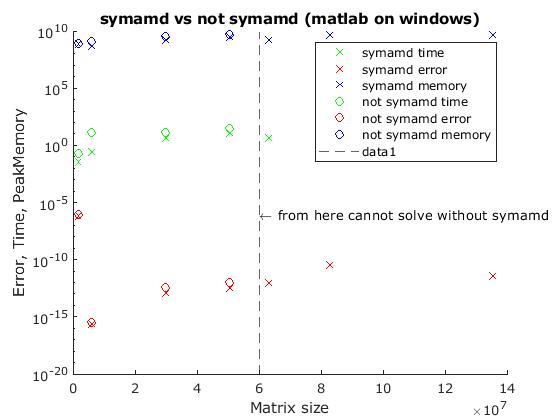
\includegraphics[width=\columnwidth]{symamdVnosym}\centering
\caption{symamd vs not symamd}\label{fig:sym}
\end{figure}
Nel grafico è riportato il confronto delle performance ottenute con e senza la permutazione basata su \emph{symamd}.
Analizzando il grafico si nota che la funzione \emph{symamd} migliora l'efficienza della decomposizione, rendendola anche possibile su matrici che altrimenti causerebbero fill-in.

\subsubsection{Matlab}
\begin{figure}[H]
    \centering
    \begin{minipage}{0.45\textwidth}
        \centering
        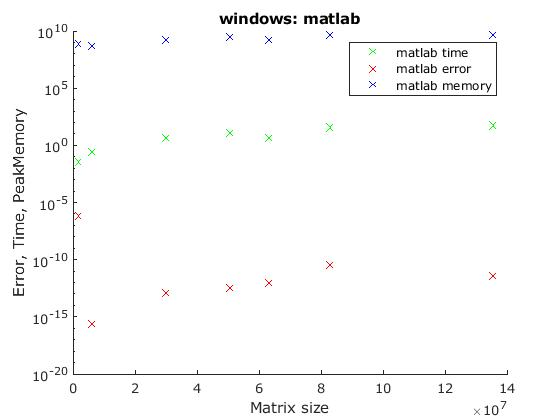
\includegraphics[width=0.9 \linewidth, height=0.3\textheight]{windowsMatlab}
    \end{minipage}
    \begin{minipage}{0.45\textwidth}
        \centering
        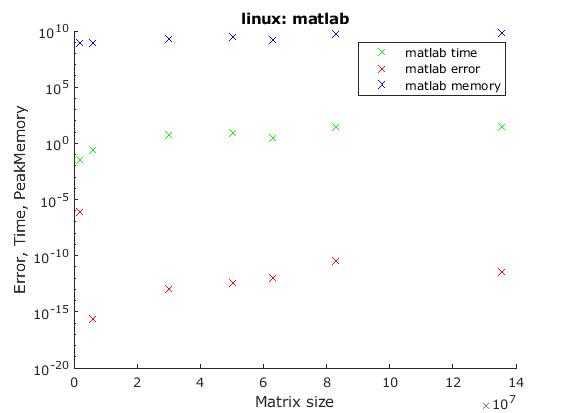
\includegraphics[width=0.9\linewidth, height=0.3\textheight]{linuxMatlab}
    \end{minipage}
\end{figure}


\begin{figure}[H]
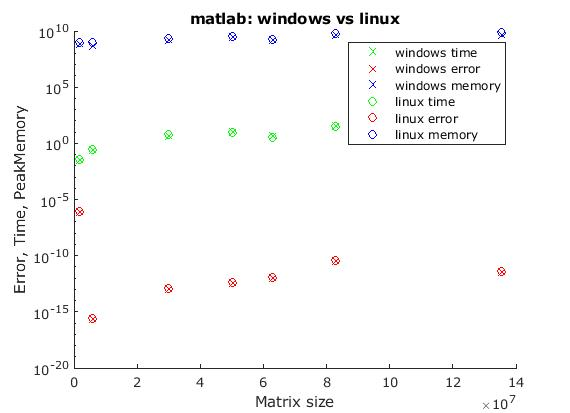
\includegraphics[width=\columnwidth]{matlabWindowsVLinux}\centering
\caption{Risultati ottenuti con Matlab}\label{fig:matlab}
\end{figure}
Prendendo in considerazione il grafico in figura \ref{fig:matlab} sulle performance di Matlab, si può notare un andamento di tutte le misure che va di pari passo per entrambi i sistemi operativi. \\
Per quanto riguarda l'errore si può notare un outsider. La matrice di dimensione inferiore (ex15) presenta il valore peggiore, mentre per le altre matrici l'errore tende a crescere all'aumentare delle dimensioni. Questo caso particolare si ripresenta anche nelle altre combinazioni di ambiente e sistema operativo.
\\\\
Si può inoltre osservare che tra i due sistemi operativi Windows è leggermente migliore nell'utilizzo di memoria.

\subsubsection{Octave}

\begin{figure}[H]
    \centering
    \begin{minipage}{0.45\textwidth}
        \centering
        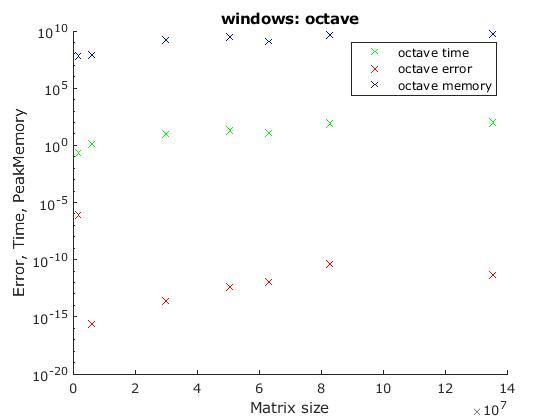
\includegraphics[width=0.9 \linewidth, height=0.3\textheight]{windowsOctave}
    \end{minipage}
    \begin{minipage}{0.45\textwidth}
        \centering
        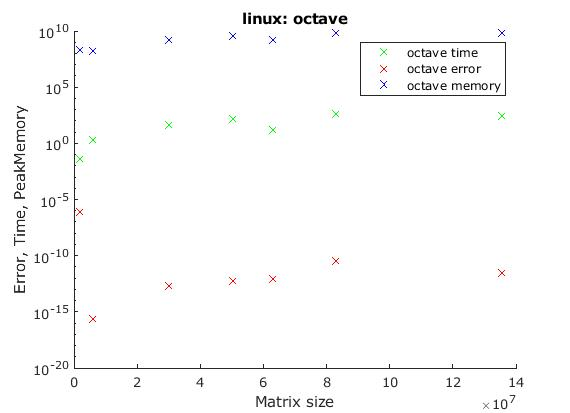
\includegraphics[width=0.9\linewidth, height=0.3\textheight]{linuxOctave}
    \end{minipage}
\end{figure}

\begin{figure}[H]
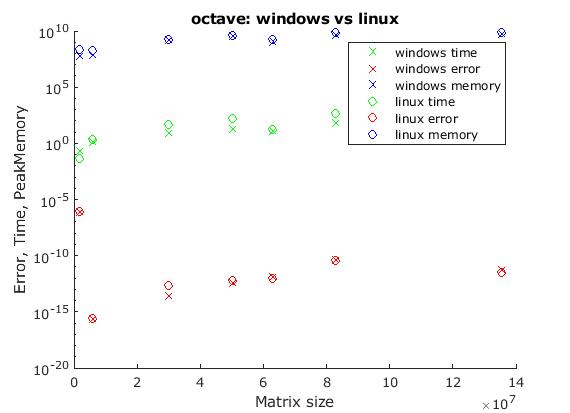
\includegraphics[width=\columnwidth]{OctaveWindowsVLinux}\centering
\caption{Risultati ottenuti con Octave}\label{fig:octave}
\end{figure}
Nel grafico sulle performance di Octave in figura \ref{fig:octave}, si possono notare differenze molto più marcate tra Linux e Windows. Per quanto riguarda l'errore, l'andamento è ambiguo e non significativo per un confronto. Per la memoria e soprattutto per il tempo, invece, è possibile notare che Windows si dimostra superiore.

\subsubsection{Linux}
\begin{figure}[H]
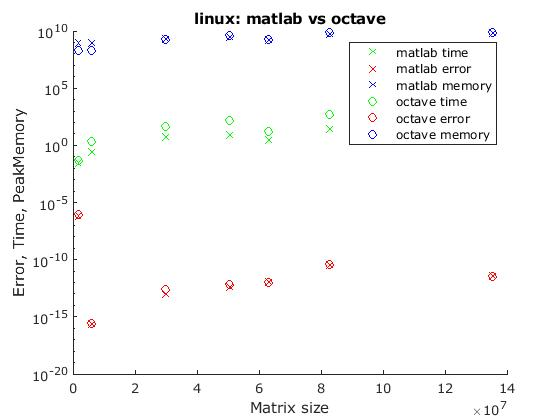
\includegraphics[width=\columnwidth]{linuxMatlabVOctave}\centering
\caption{Risultati ottenuti in Linux}\label{fig:linux}
\end{figure}
Analizzando il grafico in figura \ref{fig:linux} sui due ambienti in Linux si notano performance migliori di Matlab per quanto concerne l'errore e soprattutto il tempo. Riguardo la memoria, si può osservare come Octave abbia richiesto meno memoria per le matrici più piccole.

\subsubsection{Windows}
\begin{figure}[H]
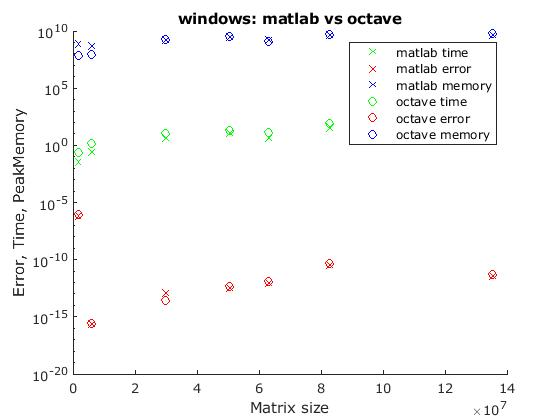
\includegraphics[width=\columnwidth]{windowsMatlabVOctave}\centering
\caption{Risultati ottenuti in Windows}\label{fig:windows}
\end{figure}

Il grafico in figura \ref{fig:windows} che confronta i due ambienti in Windows permette di osservare che Matlab ha performance nettamente superiori in termini di tempo. Per le misure di memoria ed errore non si notano particolari differenze, fatta eccezione di alcune matrici più piccole.

\subsection{Grafici aggiuntivi}\label{graficiMemoria}
Di seguito sono riportati degli ulteriori grafici che permettono di visualizzare la variazione
di memoria durante la risoluzione di ciascuno dei sistemi lineari nelle diverse combinazioni ambiente/OS. A differenza dei picchi di memoria analizzati nella sezione \ref{analisiRisultati}, ai valori è stata sottratta la quantità iniziale di memoria utilizzata dal processo in esecuzione perché ritenuta ininfluente per questo tipo di confronto. \\


\begin{figure}[H]
    \centering
    \begin{minipage}{0.45\textwidth}
        \centering
        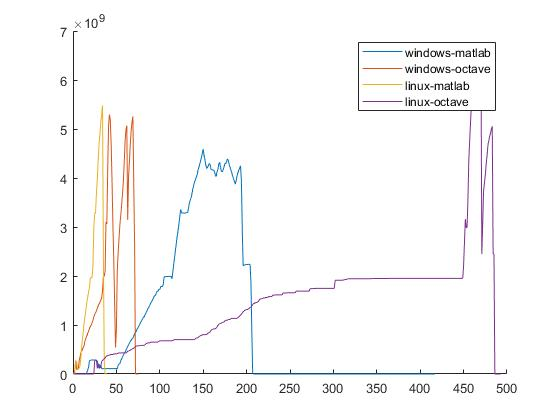
\includegraphics[width=1 \linewidth, height=0.3\textheight]{apache2Memory}
        \caption{apache2}
    \end{minipage}
    \begin{minipage}{0.45\textwidth}
        \centering
        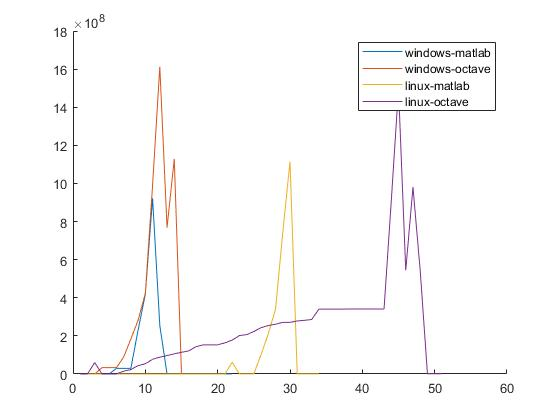
\includegraphics[width=1\linewidth, height=0.3\textheight]{cfd1Memory}
        \caption{cfd1}
    \end{minipage}
\end{figure}

\begin{figure}[H]
    \centering
    \begin{minipage}{0.45\textwidth}
        \centering
        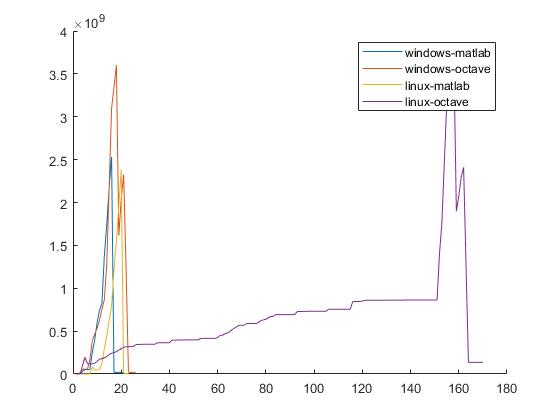
\includegraphics[width=1 \linewidth, height=0.3\textheight]{cfd2Memory}
        \caption{cfd2}
    \end{minipage}
    \begin{minipage}{0.45\textwidth}
        \centering
        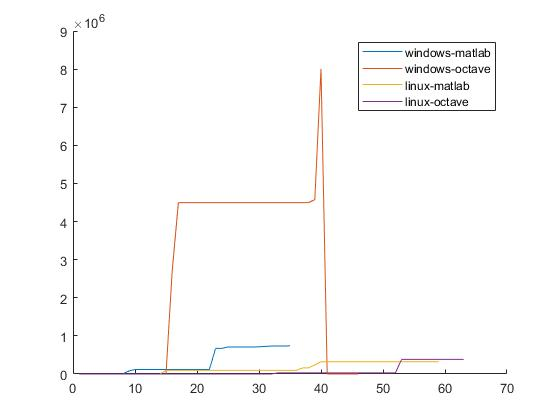
\includegraphics[width=1\linewidth, height=0.3\textheight]{ex15Memory}
        \caption{ex15}
    \end{minipage}
\end{figure}

\begin{figure}[H]
    \centering
    \begin{minipage}{0.45\textwidth}
        \centering
        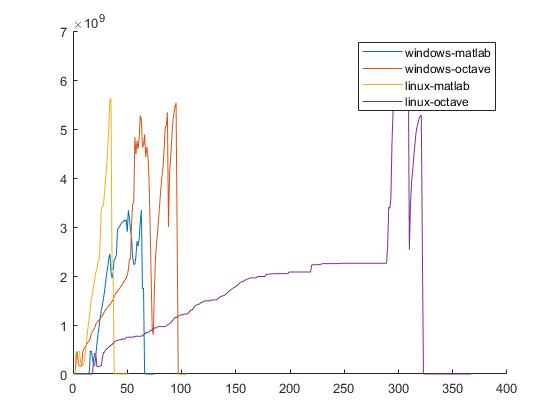
\includegraphics[width=1 \linewidth, height=0.3\textheight]{G2_circuitMemory}
        \caption{G2\_circuit}
    \end{minipage}
    \begin{minipage}{0.45\textwidth}
        \centering
        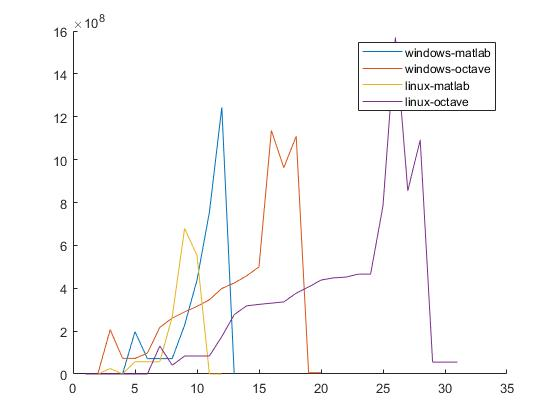
\includegraphics[width=1\linewidth, height=0.3\textheight]{parabolic_femMemory}
        \caption{parabolic\_fem}
    \end{minipage}
\end{figure}

\begin{figure}[H]
    \centering
    \begin{minipage}{0.45\textwidth}
        \centering
        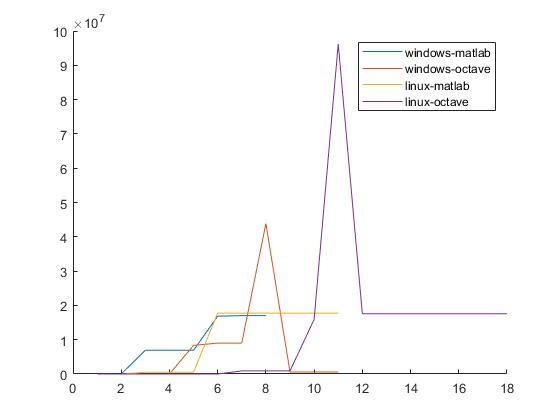
\includegraphics[width=1 \linewidth, height=0.3\textheight]{shallow_water1Memory}
        \caption{shallow\_water1}
    \end{minipage}
\end{figure}